\chapter{Server Setup and WordPress Installation}

In this project, WordPress is setup on Nginx HTTP web server running PHP preprocessor and MySQL database server. This chapter will explain on how to configure Ubuntu server, setup Nginx, PHP, MySQL database as well as WordPress.

\section{Ubuntu Server Configuration} \label{sec:ubuntu-server-configuration}
The Smart Home Lab has its own server running Ubuntu Server 16.04.2 LTS. On this server, a \ac{vm} application has been installed. This VM runs a separate virtual Ubuntu Server on the host. This VM has been allocated with its own processing power, memory and disk space. Local machine can connect to the virtual Ubuntu Server using the Wi-Fi network, SHLAB02 as shown in Figure~\ref{fig:shlab02-wlan-network}.

\begin{figure}[ht]
\caption{SHLAB02 WLAN network to connect to Ubuntu Server}
\label{fig:shlab02-wlan-network}
\centering
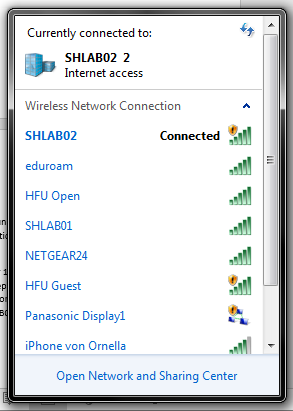
\includegraphics[height=5cm,keepaspectratio]{setup/shlab02-wlan-network.png}
\end{figure}

On the local machine, first, a \ac{ssh} key or commonly known as public/private key should be generated. This can be done using the PuTTY Key Generator application as shown in Figure~\ref{fig:putty-key-generator}. This application can be downloaded at the URL given in the footnote\footnote{http://www.chiark.greenend.org.uk/~sgtatham/putty/latest.html}. The current stable version of Putty Key Generator is 0.68, as at time of writing.

\begin{figure}[ht]
	\begin{subfigure}{.49\linewidth}
	\caption{PuTTY SSH Key Generator}
	\label{fig:putty-key-generator}
	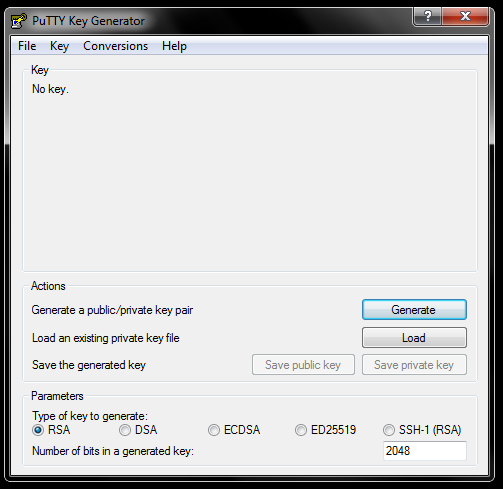
\includegraphics[width=\textwidth,keepaspectratio]{setup/putty-key-generator.png}
	\end{subfigure}
	\begin{subfigure}{.49\linewidth}
	\caption{Generating random key in PuTTY}
	\label{fig:putty-random-key}
	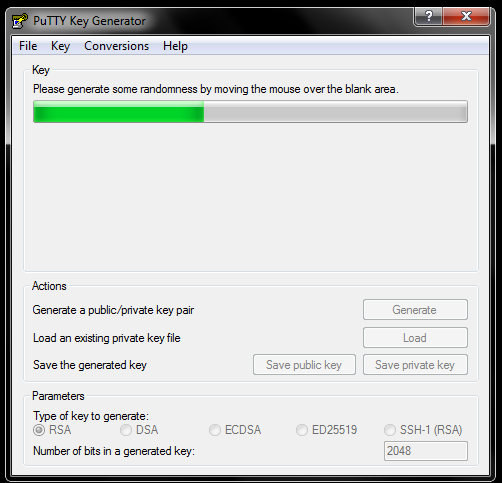
\includegraphics[width=\textwidth,keepaspectratio]{setup/putty-random-key.png}
	\end{subfigure}
\end{figure}

The keys can be generated by clicking generate button and by moving the mouse cursor randomly at the blank area as shown in Figure~\ref{fig:putty-random-key}. After that, the Key Passphrase and Confirm Passphrase must be given. This Passphrase must be noted down or remembered for future usage when connecting to the server every time. The Passphrase is \texttt{BSY2qjtu\$\#}

The generated Public Key and Private Key must be saved. The generated Public Key will be provided to the virtual Ubuntu Server running on the server. Where else the generated Private Key must be saved in the local machine that will be used to connect to the server.

\begin{figure}[ht]
\centering
	\begin{subfigure}{.49\linewidth}
	\caption{Host Name and Port}
	\label{fig:putty-connect}
	\centering
	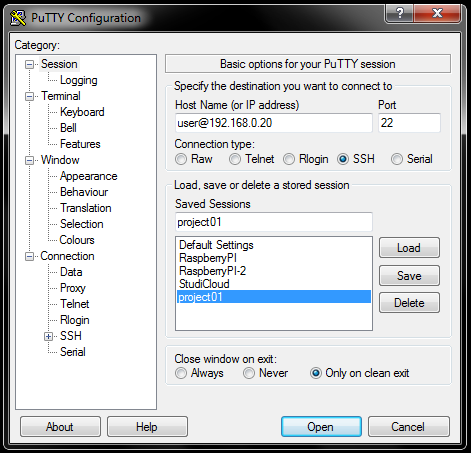
\includegraphics[width=\textwidth,keepaspectratio]{setup/putty-connect.png}
	\end{subfigure}
	\begin{subfigure}{.49\linewidth}
	\caption{Attaching Private Key}
	\label{fig:putty-private-key}
	\centering
	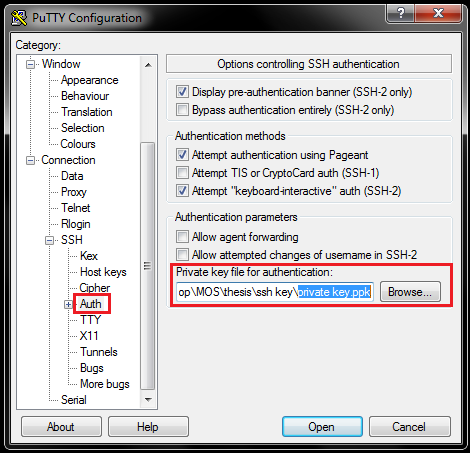
\includegraphics[width=\textwidth,keepaspectratio]{setup/putty-private-key.png}
	\end{subfigure}
\end{figure}

To connect to the server, the PuTTY application will be used. This application can be downloaded at the same link as the PuTTY Key Generator link given above. The PuTTY application will be provided with Host Name (or IP Address) of the server, which is \texttt{user@192.168.0.20} and Port number, which is\texttt{ 22} as shown in the Figure~\ref{fig:putty-connect}. After that the generated Private Key from previous step must be given in the ‘Private key file for authentication’ field as shown in Figure~\ref{fig:putty-private-key}. This field can be found under Connection > SSH > Authentication tab. Lastly ‘X11 forwarding’ must be enabled. Connection to the server can be established by pressing ‘Open’ button.

After successfully connecting, the passphrase, \texttt{BSY2qjtu\$\#} that have been entered while generating the Public/Private keys must be entered in the terminal to proceed.

\section{Nginx HTTP Server Installation} \label{sec:nginx-http-server-installation}
Nginx is a powerful, versatile and efficient HTTP or web server. Nginx web server can be installed in Ubuntu using the \texttt{apt} package.

\subsection*{Step 1: Installing Nginx}
The following has been used to install Nginx.
\begin{lstlisting}[language=sh]
$  sudo apt-get update
$  sudo apt-get install nginx
\end{lstlisting}

\subsection*{Step 2: Enabling Nginx}
The Ngnx, by default, will be configured and started running automatically after the installation. If the server runs firewall, the Nginx should be enabled manually. The Nginx will however register itself with the server firewall, which is \texttt{ufw} upon installation. The following command has to be ran in the terminal to start the Nginx manually.

\begin{lstlisting}[language=sh]
$  sudo ufw allow 'Nginx HTTP'
\end{lstlisting}

\subsection*{Step 3: Checking Nginx Status}
The status of Nginx HTTP server can be checked by using the following command.

\begin{lstlisting}[language=sh]
$  sudo ufw status
\end{lstlisting}

Running this command will output the following.
\begin{table}[ht]
\begin{tabular}{l l l}
To & Action & From \\
-- & -- & -- \\
OpenSSH & ALLOW & Anywhere \\
Nginx HTTP & ALLOW & Anywhere \\
OpenSSH  (v6) & ALLOW & Anywhere \\
Nginx HTTP (v6) & ALLOW & Anywhere \\
\end{tabular}
\end{table}

The output on the second and third column which are 'ALLOW' and 'Anywhere' respectively indicates that the Nginx is running. The successful installation of Nginx can be further tested using any web browser by entering the host's IP address, which in this case \texttt{http://192.168.0.20}. The following page will be displayed as shown in the Figure~\ref{fig:nginx-start-screen}.

\begin{figure}[ht]
\caption{Nginx Default Start Screen}
\label{fig:nginx-start-screen}
\centering
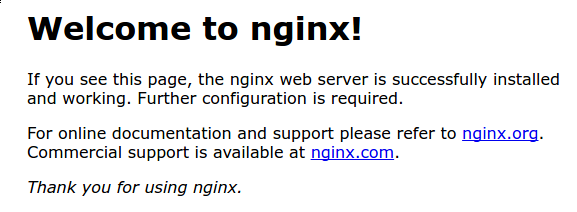
\includegraphics[height=5cm,keepaspectratio]{setup/nginx-start-screen.png}
\end{figure}


\section{MySQL Database Installation} \label{sec:mysql-database-installation}
After installing Nginx HTTP server, database server has been installed to manage the storing of the website content. In this project MySQL database server has been used.

\subsection*{Step 1: Installing MySQL}
The following command has to be entered to install MySQL database on the Ubuntu server. 
\begin{lstlisting}[language=sh]
$  sudo apt-get install mysql-server
\end{lstlisting}

During the installation, root password will be prompted or asked. Here, the password \texttt{d\_XKdEoCwX,4EnO} has been given. Here are the MySQL database credentials for future reference:
\begin{itemize*}
\item username: root
\item password: d\_XKdEoCwX,4EnO
\end{itemize*}

\subsection*{Step 2: Securing MySQL Database}
This section will discuss on how to secure the MySQL database server. To get started, the following command has to be entered in the terminal.
\begin{lstlisting}[language=sh]
$  sudo mysql_secure_installation
\end{lstlisting}

Running this command will take us through security setup of MySQL database server which consist of a series of questions. Here are the three questions and the settings that have been given for the future reference. The rest of settings have been given 'yes' as the answers.

\begin{lstlisting}[language=sh]
VALIDATE PASSWORD PLUGIN can be used to test passwords
and improve security. It checks the strength of password
and allows the users to set only those passwords which are
secure enough. Would you like to setup VALIDATE PASSWORD plugin?

Press y|Y for Yes, any other key for No: y


There are three levels of password validation policy:
LOW    Length >= 8
MEDIUM Length >= 8, numeric, mixed case, and special characters
STRONG Length >= 8, numeric, mixed case, special characters and dictionary file

Please enter 0 = LOW, 1 = MEDIUM and 2 = STRONG: 1


Using existing password for root.

Estimated strength of the password: 100
Change the password for root ? ((Press y|Y for Yes, any other key for No) : n
\end{lstlisting}

\section{PHP Preprocessor Installation} \label{sec:php-preprocessor-installation}
Nginx web server does not contain native PHP preprocessor. A package called \texttt{php-fhm}, which stand for "fastCGI process manager" must be installed on the Ubuntu server. This package tells Nginx to pass the PHP request to \texttt{php-fhm} for processing. Second package that has to be installed is \texttt{php-mysql}, which allows PHP to communicate with the database server.

\subsection*{Installing php-fpm and php-mysql}
The following command has been entered to install \texttt{php-fpm} and \texttt{php-mysql}.
\begin{lstlisting}[language=sh]
$  sudo apt-get install php-fpm php-mysql
\end{lstlisting}

\subsection*{Securing PHP configuration}
Initial installation of PHP has to be secured by commenting out the \texttt{cgi\_fix\_pathinfo} line and setting its value to \texttt{0} in the PHP configuration file, \texttt{php.ini}.

\begin{lstlisting}[language=sh]
$  sudo nano /etc/php/7,0/fpm/php.ini

/etc/php/7.0/fpm/php.ini
...
cgi\_fix\_pathinfo=0
...
\end{lstlisting}

Save and close the nano editor. Next, the PHP preprocessor has to be restarted so that the changes will take effect by entering the following command.

\begin{lstlisting}[language=sh]
$  sudo systemctl restart php7.0-fpm
\end{lstlisting}

\subsection*{Configuring Nginx to use PHP Preprocessor}
In this section, a few settings changes on the Nginx will be shown in order to ask Nginx to use PHP preprocessor. The server settings of Nginx can be opened using the following command.

\begin{lstlisting}[language=sh]
$  sudo nano /etc/nginx/sites-available/default
\end{lstlisting}

After opening the server settings, \texttt{index.php} has to be added to index line in the server block. In addition to that, two new block \texttt{location \~\textbackslash php\$} and \texttt{location \~/\textbackslash .ht \{} has to be introduced.

\begin{lstlisting}[language=sh]
server {
    ...
    index index.php

    location ~ \.php$ {
        include snippets/fastcgi-php.conf;
        fastcgi_pass unix:/run/php/php7.0-fpm.sock;
    }

    location ~ /\.ht {
        deny all;
    }
}
\end{lstlisting}

After adding those lines to the Nginx configuration files, the configuration file has to be checked for error. If no error is reported, the web server can be restarted safely as shown below.

\begin{lstlisting}[language=sh]
$  sudo nginx -t
$  sudo systemctl reload nginx
\end{lstlisting}

\subsection*{Testing PHP Preprocessor}
The installation and configuration of PHP preprocessor can be tested by introducing \texttt{info.php} to the server root directory. A PHP information file can be created by using the following command.

\begin{lstlisting}[language=sh]
$  sudo nano /var/www/html/info.php
\end{lstlisting}

In the PHP file, following lines have to be added. After adding those lines, save and close the file.
\begin{lstlisting}[language=PHP]
<?php
    phpinfo();
\end{lstlisting}

Now the PHP preprocessor can be tested using web browser by entering the URL, \texttt{http://192.168.0.20/info.php}. After testing the PHP preprocessor, it is important that \texttt{info.php} file has to be deleted to prevent anyone from learning the PHP configurations.

\section{WordPress Installation} \label{sec:wordpress-installation}
After installing Nginx, PHP and MySQL, we can begin with WordPress installation. Please make sure to log in into server-side using PuTTY. Before we can install the WordPress, there are few settings / configurations that have to be done, which includes:
\begin{itemize*}
\item Setting up database table and database user
\item Configuring Nginx server
\item Installing additional PHP modules to handle WordPress
\item Generating secret keys
\item Downloading latest stable version of WordPress
\item Configuring WordPress
\end{itemize*}

\subsection*{Step 1: Creating MySQL Database and User}

First, we need to prepare a database table and user in the installed MySQL. The database table and user will then be used by WordPress to store data and access them.

Start MySQL database by issuing the following command:

\begin{lstlisting}[language=sh]
$ mysql -u root -p
\end{lstlisting}

Enter the password \texttt{d\_XKdEoCwX,4EnO} for the user \texttt{root} when prompted.

Create a new database table \texttt{wordpress} by issuing following command. And don't forget the semicolon at the end of the line.
\begin{lstlisting}[language=SQL]
mysql > CREATE DATABASE wordpress DEFAULT CHARACTER SET utf8 COLLATE utf8_unicode_ci;
\end{lstlisting}

Next, create a new user to operate the above created \texttt{wordpress} database. The following command will create a new user \texttt{wordpressuser} with password \texttt{ABcd1234\#}.

\begin{lstlisting}[language=SQL]
myql > GRANT ALL ON wordpress.* TO 'wordpressuser'@'localhost' IDENTIFIED BY 'ABcd1234#';
\end{lstlisting}

This will create the new user with given password, as well as granting the user the all accesses to the database \texttt{wordpress}. Finally, flush the privileges so that the MySQL aware of the changes we have made and exit MySQL.

\begin{lstlisting}[language=SQL]
mysql > FLUSH PRIVILEGES;
mysql > EXIT;
\end{lstlisting}


\subsubsection*{Step 2: Adjust Nginx's Configuration}
There are two modifications that have to be made to the Nginx web server to handle WordPress correctly:
\begin{enumerate}
\item Instruct server not to log requests for the static files with extensions such as .css, .gif etc.
\item Insert \texttt{index.php} into \texttt{try\_files}
\end{enumerate}

Open the Nginx configuration file using \texttt{sudo} privileges:
\begin{lstlisting}[language=sh]
$ sudo nano /etc/nginx/sites-available/default
\end{lstlisting}

We can request server not to log requests to the static files by issuing command {\tt log\_not\_found off}. It is a best practice not to log requests to static files.

\begin{lstlisting}[language=sh]
server {
	...
	location = /favicon.ico {
		log_not_found off;
		access_log off
	}
	location = /robot.txt {
		log_not_found off;
		access_log off;
		allow all;
	}
	location ~* \.(css|gif|ico|jpeg|jpg|js|png)$ {
		expires max;
		log_not_found off;
	}
	...
}
\end{lstlisting}

For the second task, passing \texttt{index.php} as \texttt{try\_files} is done so that the server will return home page instead of 404 error as a default option. To do this, following line has to put inside \texttt{location /} block.

\begin{lstlisting}[language=sh]
server {
	...
	location / {
		#try_files $uri $uri/ =404;
		try_files $uri $uri/ /index.php$is_args$args;
	}
	...
}
\end{lstlisting}

When these changes have been made, save the configuration file and exit \texttt{nano} editor by pressing \texttt{Ctrl-x}. Check for the syntax errors of the new configurations. If no error is been reported, restart the Nginx.

\begin{lstlisting}[language=sh]
$ sudo nginx -t
$ sudo systemctl reload nginx
\end{lstlisting}

\subsubsection*{Step 3: Installing additional PHP extensions}
PHP preprocessor has been installed and setup with minimal setting in the previous section. Here, additional modules or extensions will be installed, which is required by WordPress \cite{SugarHill.2016}. Use to following command to install the required additional extensions:

\begin{lstlisting}[language=sh]
$ sudo apt-get update
$ sudo apt-get install php-curl php-gd php-mbstring php-mcrypt php-xml php-xmlrpc
\end{lstlisting}

After finish installing the extensions, restart the \texttt{php-fpm} process.
\begin{lstlisting}[language=sh]
$ sudo systemctl restart php7.0-fpm
\end{lstlisting}

\subsubsection*{Step 4: Generating secret keys}
Secret keys have to be generated to provide security for the WordPress. The secret keys are provided by WordPress through their secure key generator. To get secret keys from WordPress key generator, issue the following command on the terminal:

\begin{lstlisting}[language=sh]
$ curl -s https://api.wordpress.org/secret-key/1.1/salt
\end{lstlisting}

Or another workaround is to use the web browser. Enter the URL \texttt{https://api.wordpress.org/secret-key/1.1/salt} and press enter. Save the generated secret keys, which must be used in the next step.


\subsubsection*{Step 5: Downloading WordPress}
Download the latest version of stable WordPress from https://wordpress.org website. After downloading, extract the downloaded content.

\begin{lstlisting}[language=sh]
$ cd /tmp
$ curl -o https://wordpress.org/latest.tar.gz
$ tar xzvf latest.tar.gz
\end{lstlisting}

By default, WordPress has provided a sample copy of the WordPress configuration file. This file can be found under directory and file name \texttt{tmp/wordpress/wp-config-sample.php}.

Copy the provided configuration file to used in our website. And Create a new directory \texttt{upgrade}, so that WordPress can upgrade its software in the future without any permission issue.
\begin{lstlisting}[language=sh]
$ cp /tmp/wordpress/wp-config-sample.php /tmp/wordpress/wp-config.php
$ mkdir /tmp/wordpress/wp-content/upgrade
\end{lstlisting}

Finally, copy the contents into root server directory. This are the contents used by the Nginx web server to serve when request is made to the website.
\begin{lstlisting}[language=sh]
$ sudo cp -a /tmp/wordpress/. /var/www/html
\end{lstlisting}

\subsubsection*{Step 6: Configuring WordPress}
Open the WordPress configuration file:
\begin{lstlisting}[language=sh]
$ nano /var/www/html/wp-config.php
\end{lstlisting}

In the file, find the 'secret key' section, which appears as follow and paste the generated secret keys from Step 4.
\begin{lstlisting}[language=sh]
...
define('AUTH_KEY', 'put your unique phrase here');
define('SECURE_AUTH_KEY', 'put your unique phrase here');
define('LOGGED_IN_KEY', 'put your unique phrase here');
define('NONCE_KEY', 'put your unique phrase here');
define('AUTH_SALT', 'put your unique phrase here');
define('SECURE_AUTH_SALT', 'put your unique phrase here');
define('LOGGED_IN_SALT', 'put your unique phrase here');
define('NONCE_SALT', 'put your unique phrase here');
...
\end{lstlisting}


After pasting the generated secret keys, the MySQL database credentials have to be given. These credentials have been created in the Step 1.
\begin{lstlisting}[language=sh]
...
define('DB_NAME', 'wordpress');

/** MySQL database username */
define('DB_USER', 'wordpressuser');

/** MySQL database password */
define('DB_PASSWORD', 'ABcd1234#');
\end{lstlisting}

Lastly, we need to give permission to Nginx web server to write where it needs to. Otherwise, WordPress will be asking FTP credentials when any actions need to be performed. This can be done through following setting:
\begin{lstlisting}[language=sh]
define('FS_METHOD', 'direct');
\end{lstlisting}

Save the \texttt{wp-config.php} file and exit the nano editor.

\subsubsection*{Step 7: Complete WordPress Installation}
We need to complete the WordPress installation now through the web browser. Open the web browser and enter the URL \texttt{192.168.0.20}. First, we need to select the language.

\begin{figure}[ht]
\caption{WordPress language selection}
\label{fig:wordpress-language-selection}
\centering
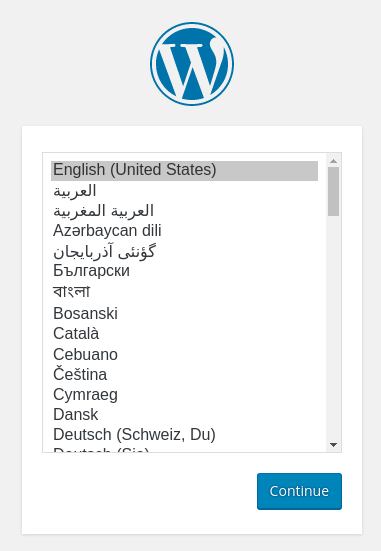
\includegraphics[height=5cm,keepaspectratio]{setup/language-selection.png}
\end{figure}

After that, we need to provide a few information on the main setup page such as \emph{Site Title}, \emph{Username}, \emph{Password} and \emph{Email}.

\begin{figure}[ht]
\caption{Main WordPress setup page}
\centering
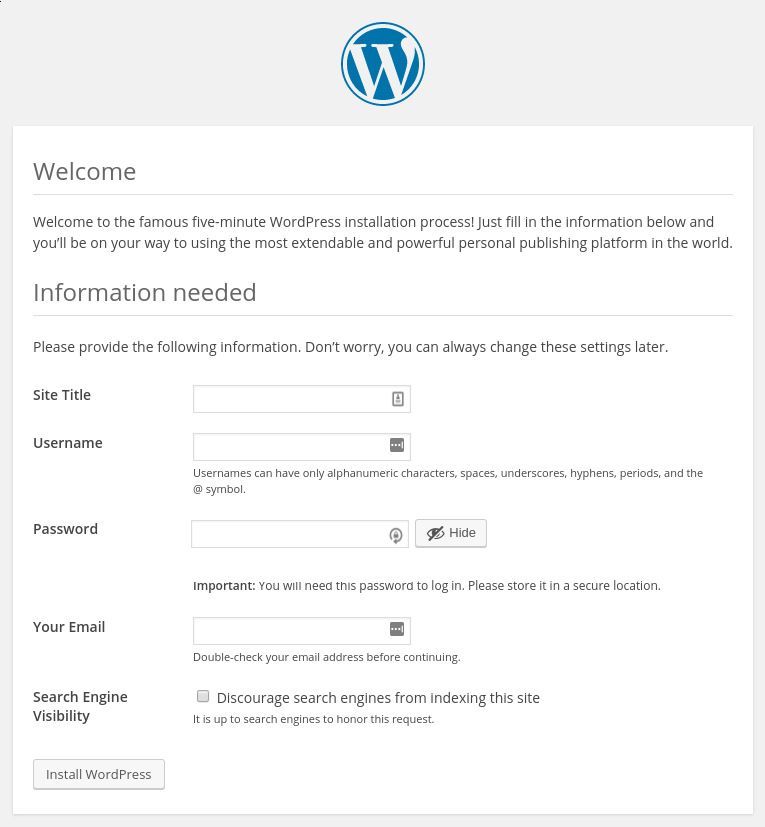
\includegraphics[height=6cm,keepaspectratio]{setup/main-wp-setup.png}
\end{figure}

These are information given on the page shown above:
\begin{itemize*}
\item Site Title: Smart Home Lab
\item Username: ashiqmoh
\item Password: oSm0cCCAguIMsalrZd(\#2i5(
\item Email: ashiqmoh@192.168.0.20
\end{itemize*}

The installation can be completed by clicking 'Install WordPress' button. Upon installation, the administration side of the website can be accessed by entering following URL:
\begin{lstlisting}
http://192.168.0.20/wp-admin
\end{lstlisting}

Provide the username and password stated above and login. The administration side of the website appears as shown in the figure below.

\begin{figure}[ht]
\caption{Administation page of WordPress}
\centering
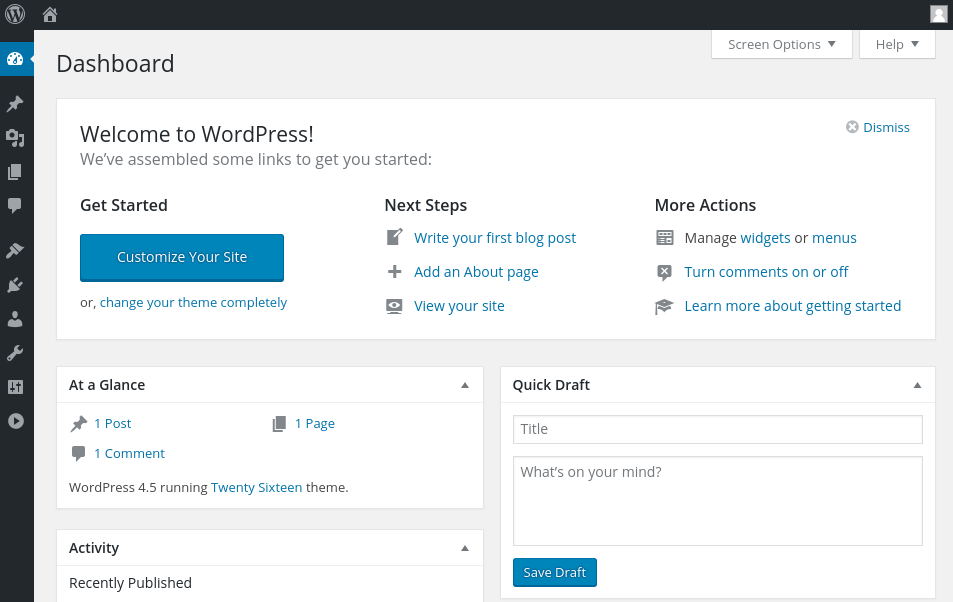
\includegraphics[height=7cm,keepaspectratio]{setup/wp-admin-page.png}
\end{figure}

\section{Routing WordPress to external URL} \label{sec:routing-wordpress-to-external-url}
The website i.e. WordPress, that has been installed inside one of the virtual machine in the Smart Home Lab physical server, by default can be accessed internally only through the \ac{ip} address \texttt{192.168.0.20}. To make the website accessible from external network through an \ac{url} address, the following steps have to be done.

Go to the general settings of the WordPress by clicking \scalerel*{
\includegraphics{setup/settings-button.png}}{B} button from the left navigation menus. Then, click on the \scalerel*{
\includegraphics{setup/general-button.png}}{B} button from the sub-menus.

Here, the following fields can be changed from \texttt{192.168.0.20} to the desired \ac{url} address:
\begin{itemize*}
\item WordPress Address (URL)
\item Site Address (URL)
\end{itemize*}

Both the text fields have been changed to the URL address:
\begin{lstlisting}
http://web.smarthome.hs-furtwangen.de
\end{lstlisting}

By doing this, the website can be accessed externally.

\section{Restrict Website Access to Internal Network}
The access to the website from external network can be revoked and restrict it to be accessible only from within the lab network by reversing the process described in the Section~\ref{sec:routing-wordpress-to-external-url}. The \emph{WordPress Address (URL)} and \emph{Site Address (URL)} text fields have to be changed to the \ac{ip} address \texttt{192.168.0.20}.


